\documentclass[aspectratio=169]{beamer}

% ── Professor's UofT Template ──────────────────────────────────
\usetheme{CambridgeUS}
\usecolortheme{beaver}

% --- U of T BRAND COLORS (same as other CSC415 lectures) ---
\definecolor{UofTBlue}{RGB}{0, 42, 92}
\definecolor{UofTSky}{RGB}{0, 127, 163}
\definecolor{UofTSilver}{RGB}{226, 231, 235}

\setbeamercolor{palette primary}{bg=UofTBlue, fg=white}
\setbeamercolor{palette secondary}{bg=UofTSky, fg=white}
\setbeamercolor{palette tertiary}{bg=UofTBlue, fg=white}

\setbeamercolor{title}{bg=UofTBlue, fg=white}
\setbeamercolor{subtitle}{fg=UofTSilver}
\setbeamercolor{frametitle}{bg=white, fg=UofTBlue}
\setbeamercolor{structure}{fg=UofTBlue}
\setbeamercolor{item}{fg=UofTSky}

\setbeamercolor{block title}{bg=UofTBlue, fg=white}
\setbeamercolor{block body}{bg=UofTSilver, fg=black}
\setbeamercolor{block title alerted}{bg=red!70!black, fg=white}
\setbeamercolor{block body alerted}{bg=red!10, fg=black}
\setbeamercolor{block title example}{bg=UofTSky, fg=white}
\setbeamercolor{block body example}{bg=UofTSky!10, fg=black}

\setbeamertemplate{headline}{
  \begin{beamercolorbox}[ht=3.5ex,dp=1.125ex,leftskip=12pt,rightskip=12pt]{section in head/foot}
    \usebeamerfont{section in head/foot}\insertsection
  \end{beamercolorbox}
}

\setbeamertemplate{navigation symbols}{}

% Accent colors for highlights
\definecolor{AccentOrange}{RGB}{230, 126, 34}
\definecolor{SuccessGreen}{RGB}{39, 174, 96}
\definecolor{DangerRed}{RGB}{192, 57, 43}

% Packages
\usepackage[utf8]{inputenc}
\usepackage[T1]{fontenc}
\usepackage{amsmath,amssymb}
\usepackage{graphicx}
\usepackage{booktabs}
\usepackage{multirow}
\usepackage{xcolor}
\usepackage{adjustbox}
\usepackage{tikz}
\usepackage{caption}
\usetikzlibrary{calc,arrows.meta,positioning,shapes.geometric}
\setbeamerfont{caption}{size=\footnotesize}

% Custom commands
\newcommand{\highlight}[1]{\textcolor{AccentOrange}{\textbf{#1}}}
\newcommand{\good}[1]{\textcolor{SuccessGreen}{\textbf{#1}}}
\newcommand{\bad}[1]{\textcolor{DangerRed}{\textbf{#1}}}

\graphicspath{{figures/}}

\title[Auxiliary Losses for Visual RL]{Auxiliary Representation Losses for\\Distractor-Robust Visual RL}
\subtitle{Extending DrQ-v2 with Lightweight Self-Supervised Objectives}
\author{Bangcheng Wang \and Kean Chen}
\institute[]{University of Toronto --- CSC415: Introduction to Reinforcement Learning}
\date{Winter 2026}

% Custom title page (from template)
\makeatletter
\setbeamertemplate{title page}{
  \vbox{}
  \vfill
  \begingroup
    \centering
    \textcolor{UofTBlue}{\textbf{\Large University of Toronto}}\\[1.5em]
    \begin{beamercolorbox}[sep=12pt,center,rounded=true,shadow=true]{title}
      \usebeamerfont{title}\inserttitle\par%
      \ifx\insertsubtitle\@empty%
      \else%
        \vskip0.5em%
        {\usebeamerfont{subtitle}\usebeamercolor[fg]{subtitle}\insertsubtitle\par}%
      \fi%
    \end{beamercolorbox}%
    \vskip1em\par
    {\usebeamerfont{author}\insertauthor}\vskip0.5em
    {\usebeamerfont{institute}\insertinstitute}\vskip0.5em
    {\usebeamerfont{date}\insertdate}\vskip0.5em
  \endgroup
  \vfill
}
\makeatother

\begin{document}

% ==============================================================
% TITLE SLIDE
% ==============================================================
{
\setbeamertemplate{footline}{}
\frame{\titlepage}
}

% ==============================================================
% CONTENTS
% ==============================================================
\begin{frame}{Contents}

\begin{columns}[T]
\begin{column}{0.48\textwidth}
\textbf{Part I --- Bangcheng}
\begin{enumerate}
    \item Background \& Motivation
    \item Research Question
    \item Method: Mod A \& Mod B
\end{enumerate}
\end{column}
\begin{column}{0.48\textwidth}
\textbf{Part II --- Kean}
\begin{enumerate}
    \setcounter{enumi}{3}
    \item Experimental Setup
    \item Main Results (3 tasks)
    \item Analysis \& Interpretation
    \item Conclusion \& Future Work
\end{enumerate}
\end{column}
\end{columns}

\vspace{1em}
\centering
{\small 10 min presentation + 5 min Q\&A}

\end{frame}

% ==============================================================
\section{Background}

\begin{frame}{Background: Learning RL from Pixels}
% Speaker: Bangcheng (~45 sec)

\small
\begin{columns}[T]
\begin{column}{0.55\textwidth}
\textbf{The challenge:}\\
Visual RL gets \highlight{raw 84$\times$84 pixels} (21,168 dims),\\
not clean state vectors.

\vspace{0.2em}
\textbf{Solution: learn an encoder}
\begin{itemize}\setlength{\itemsep}{1pt}
    \item Pixels $\to$ 50-dim features. \highlight{Encoder quality = agent quality}
    \item Actor \& Critic both depend on this representation
\end{itemize}

\vspace{0.2em}
\textbf{How to train it?}
\begin{itemize}\setlength{\itemsep}{1pt}
    \item DrQ-v2: only through critic loss
    \item Our idea: add \highlight{auxiliary losses} as extra signals
\end{itemize}
\end{column}
\begin{column}{0.42\textwidth}
\centering
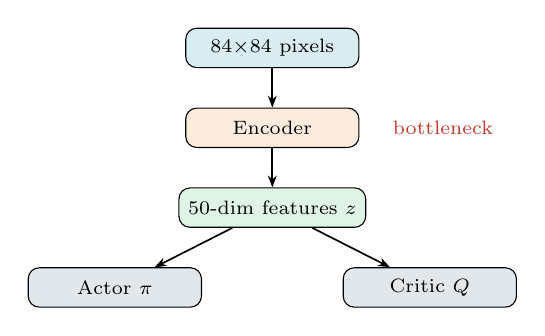
\begin{tikzpicture}[
    node distance=0.4cm,
    box/.style={draw, rounded corners, minimum width=2.2cm, minimum height=0.5cm, font=\scriptsize, fill=UofTSilver},
    arr/.style={-{Stealth[length=1.5mm]}, semithick}
]
    \node[box, fill=UofTSky!15] (pixels) {84$\times$84 pixels};
    \node[box, below=0.5cm of pixels, fill=AccentOrange!15] (enc) {Encoder};
    \node[box, below=0.5cm of enc, fill=SuccessGreen!15] (z) {50-dim features $z$};
    \node[box, below left=0.5cm and -0.3cm of z] (actor) {Actor $\pi$};
    \node[box, below right=0.5cm and -0.3cm of z] (critic) {Critic $Q$};

    \draw[arr] (pixels) -- (enc);
    \draw[arr] (enc) -- (z);
    \draw[arr] (z) -- (actor);
    \draw[arr] (z) -- (critic);

    \node[right=0.3cm of enc, font=\scriptsize\color{DangerRed}] {bottleneck};
\end{tikzpicture}

\vspace{0.3em}
{\footnotesize If the encoder fails to extract\\task-relevant features, both\\actor and critic will fail.}
\end{column}
\end{columns}
\end{frame}

% ==============================================================

\begin{frame}[shrink=3]{DrQ-v2: Strong but Fragile}
% Speaker: Bangcheng (~60 sec)

\small
\begin{columns}[T]
\begin{column}{0.55\textwidth}
\textbf{DrQ-v2} (Yarats et al., ICLR 2022):
\begin{itemize}\setlength{\itemsep}{1pt}
    \item \highlight{DDPG} + random-shift augmentation ($\pm 4$\,px)
    \item Encoder learns to ignore small camera movements
    \item No auxiliary losses, no momentum encoders
    \item \good{SOTA on clean DMC tasks}
\end{itemize}

\vspace{0.2em}
\begin{alertblock}{The Problem}
Under \bad{video distractors}, cartpole drops \bad{$\sim$11\%} ($839 \to 747$). Random-shift cannot teach ``ignore moving backgrounds''.
\end{alertblock}
\end{column}
\begin{column}{0.42\textwidth}
\centering
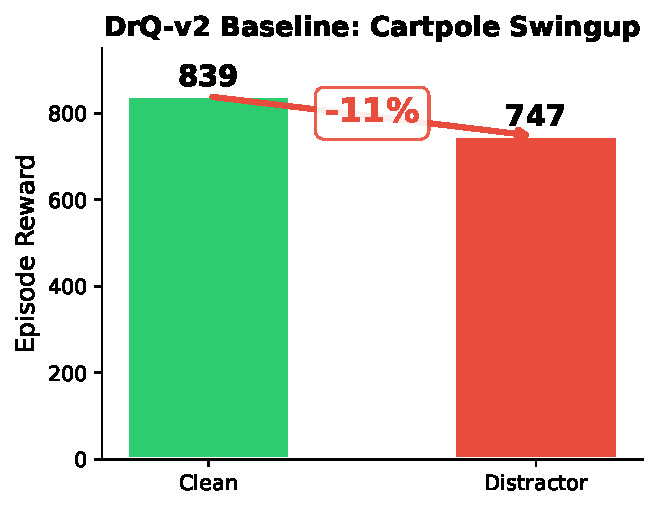
\includegraphics[width=\textwidth]{baseline_drop.pdf}

\vspace{0.3em}
{\footnotesize Clean (blue) vs.\ Distractor (red)\\Cartpole: $839 \to 747$ ($-11\%$)}
\end{column}
\end{columns}
\end{frame}

% ==============================================================
\section{Research Question}

\begin{frame}{Research Question}
% Speaker: Bangcheng (~40 sec)
% SAY: Our question is simple. Can we add a small loss to fix this?
% SAY: We tested two ideas from our Assignment 1 reviews.

\begin{center}
\large\color{UofTBlue}
\textbf{Can lightweight auxiliary losses improve DrQ-v2's\\distractor robustness without changing its architecture?}
\end{center}

\vspace{0.3em}

\begin{block}{Our Approach}
\vspace{-0.2em}
Two auxiliary losses from our Assignment~1 paper reviews, added to the critic:
\vspace{-0.5em}
\[
\mathcal{L}_{\text{total}} = \underbrace{\mathcal{L}_{\text{critic}}}_{\text{original DrQ-v2}} + \;\alpha \cdot \underbrace{\mathcal{L}_{\text{aux}}}_{\text{our addition}}
\]
\vspace{-0.8em}
\end{block}

\vspace{0.2em}
\begin{columns}[c]
\begin{column}{0.46\textwidth}
\centering
\highlight{Mod\,A} --- \textbf{Task-agnostic}\\[0.2em]
{\small ``Same state, different views\\$\to$ same encoding''}\\[0.1em]
{\footnotesize Inspired by SimSiam (self-supervised)}
\end{column}
\begin{column}{0.08\textwidth}
\centering vs.
\end{column}
\begin{column}{0.46\textwidth}
\centering
\highlight{Mod\,B} --- \textbf{Task-aware}\\[0.2em]
{\small ``Similar Q-values\\$\to$ similar encoding''}\\[0.1em]
{\footnotesize Inspired by bisimulation metrics}
\end{column}
\end{columns}
\end{frame}

% ==============================================================
\section{Method}

\begin{frame}{Mod A: Consistency Regularizer --- Intuition}
% Speaker: Bangcheng (~40 sec)
% SAY: Here is the key idea behind Mod A. Very simple.

\begin{center}
\large\color{UofTBlue}
\textbf{``If two views show the same physical state,\\their encodings must match.''}
\end{center}

\vspace{0.3em}
\small
\begin{columns}[T]
\begin{column}{0.55\textwidth}
\textbf{Step by step:}
\begin{enumerate}\setlength{\itemsep}{3pt}
    \item Take one observation from the replay buffer
    \item Apply two \emph{different} random shifts ($\pm 4$\,px)
    \item Encode both shifted versions: get $z_1$ and $z_2$
    \item Loss = MSE($z_1$, $z_2$): \highlight{force them to match}
\end{enumerate}

\vspace{0.3em}
\textbf{Why does this help with distractors?}\\
The encoder learns: ``if the physics didn't change, my output shouldn't change''. This generalizes beyond pixel shifts --- it encourages ignoring \emph{any} visual variation that doesn't affect the task.
\end{column}
\begin{column}{0.42\textwidth}
\centering
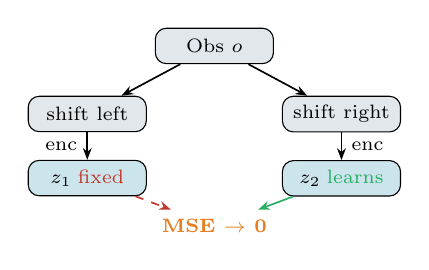
\begin{tikzpicture}[
    node distance=0.5cm,
    box/.style={draw, rounded corners, minimum width=1.5cm, minimum height=0.45cm, font=\scriptsize, fill=UofTSilver},
    arr/.style={-{Stealth[length=1.5mm]}, semithick}
]
    \node[box] (obs) {Obs $o$};
    \node[box, below left=0.4cm and 0.1cm of obs] (f1) {shift left};
    \node[box, below right=0.4cm and 0.1cm of obs] (f2) {shift right};
    \node[box, below=0.35cm of f1, fill=UofTSky!20] (z1) {$z_1$\;{\scriptsize\textcolor{DangerRed}{fixed}}};
    \node[box, below=0.35cm of f2, fill=UofTSky!20] (z2) {$z_2$\;{\scriptsize\textcolor{SuccessGreen}{learns}}};
    \node[below=0.4cm of $(z1)!0.5!(z2)$, font=\scriptsize\bfseries, text=AccentOrange] (mse) {MSE $\to$ 0};

    \draw[arr] (obs) -- (f1);
    \draw[arr] (obs) -- (f2);
    \draw[arr] (f1) -- node[left, font=\scriptsize]{enc} (z1);
    \draw[arr] (f2) -- node[right, font=\scriptsize]{enc} (z2);
    \draw[arr, dashed, DangerRed] (z1) -- (mse);
    \draw[arr, SuccessGreen] (z2) -- (mse);
\end{tikzpicture}

\vspace{0.3em}
{\footnotesize Same physical state\\$\Rightarrow$ same encoding}
\end{column}
\end{columns}
\end{frame}

% ==============================================================

\begin{frame}{Mod A: Technical Details}
% Speaker: Bangcheng (~40 sec)
% SAY: The formula looks complex but the idea is just MSE between two views.

\vspace{-0.2em}
\begin{equation*}
\mathcal{L}_{\text{consistency}} = \mathbb{E}_{o \sim \mathcal{B}} \left[\left\| \operatorname{sg}[\operatorname{enc}(f_1(o))] - \operatorname{enc}(f_2(o)) \right\|_2^2 \right]
\end{equation*}
\vspace{-0.3em}

\small
\begin{columns}[T]
\begin{column}{0.52\textwidth}
\begin{exampleblock}{\good{Three Practical Advantages}}
\begin{enumerate}\setlength{\itemsep}{3pt}
    \item \good{Zero overhead}: DrQ-v2 already computes $z_1, z_2$ for actor/critic. We just add one MSE on top.
    \item \good{No extra network}: just one loss term added to the critic.
    \item \good{One hyperparameter}: $\alpha = 0.1$. Robust across $[0.01, 1.0]$ (100$\times$ range, only 4\% performance variation).
\end{enumerate}
\end{exampleblock}
\end{column}
\begin{column}{0.45\textwidth}
\begin{alertblock}{Why stop-gradient (sg)?}
Without it, the encoder would \bad{cheat}:\\
set all outputs to zero $\to$ $z_1 = z_2 = \mathbf{0}$.

Loss = 0, but representation is \bad{useless}.\\
This is called \highlight{representation collapse}.

\vspace{0.2em}
\good{Fix}: freeze $z_1$ (stop-gradient).\\
$z_2$ must match a \emph{meaningful} target,\\not just collapse to zero.
\end{alertblock}
\end{column}
\end{columns}
\end{frame}

% ==============================================================
\begin{frame}{Mod B: Task-Conditional Contrastive Loss --- Intuition}
% Speaker: Bangcheng (~40 sec)
% SAY: Mod B takes a completely different approach. Instead of comparing views of the same image, it compares different states.

\begin{center}
\large\color{UofTBlue}
\textbf{``States that play a similar role in the task\\should have similar encodings.''}
\end{center}

\vspace{0.3em}
\small
\begin{columns}[T]
\begin{column}{0.52\textwidth}
\textbf{How it defines ``similar role'':}
\begin{itemize}\setlength{\itemsep}{3pt}
    \item Use \highlight{Q-values} as a proxy for behavioral similarity
    \item If $|Q_i - Q_j| < \epsilon$: these states are \good{positive pairs}\\(pull their encodings together)
    \item If $|Q_i - Q_j|$ is large: these are \bad{negative pairs}\\(push their encodings apart)
\end{itemize}

\vspace{0.2em}
\textbf{vs.\ CURL} (also contrastive):\\
CURL defines positives by \emph{visual} augmentation.\\
Mod B defines positives by \emph{task behavior} (Q-values).\\
$\Rightarrow$ Mod B is \highlight{task-aware}, not just vision-aware.
\end{column}
\begin{column}{0.45\textwidth}
\centering
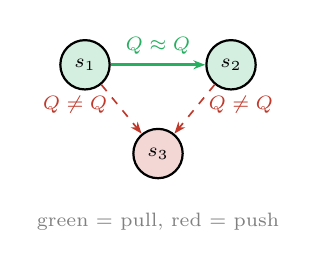
\begin{tikzpicture}[
    node distance=0.3cm,
    state/.style={circle, draw, minimum size=0.6cm, font=\scriptsize, thick},
    arr/.style={-{Stealth[length=1.5mm]}, semithick}
]
    \node[state, fill=SuccessGreen!20] (a) {$s_1$};
    \node[state, fill=SuccessGreen!20, right=1.2cm of a] (b) {$s_2$};
    \node[state, fill=DangerRed!20, below=0.8cm of $(a)!0.5!(b)$] (c) {$s_3$};

    \draw[arr, SuccessGreen, very thick] (a) -- node[above, font=\scriptsize]{$Q \approx Q$} (b);
    \draw[arr, DangerRed, dashed] (a) -- node[left, font=\scriptsize, pos=0.4]{$Q \neq Q$} (c);
    \draw[arr, DangerRed, dashed] (b) -- node[right, font=\scriptsize, pos=0.4]{$Q \neq Q$} (c);

    \node[below=0.3cm of c, font=\scriptsize\color{gray}] {green = pull, red = push};
\end{tikzpicture}

\vspace{0.5em}
{\footnotesize This is a lightweight proxy\\for \highlight{bisimulation metrics}:\\states that ``behave the same''\\should ``look the same'' to the encoder.}
\end{column}
\end{columns}
\end{frame}

% ==============================================================
\begin{frame}[shrink=3]{Mod B: Technical Details \& Risk}
% Speaker: Bangcheng (~40 sec)
% SAY: This sounds good in theory. But there are two serious problems.

\vspace{-0.3em}
{\small
\begin{equation*}
\mathcal{L}_{\text{task}} = -\log \frac{\exp(\operatorname{sim}(z_i, z_j) / \tau)}{\sum_{k \neq i} \exp(\operatorname{sim}(z_i, z_k) / \tau)}, \;\; (i,j)\text{ pos.\ if } |Q_i - Q_j| < \epsilon
\end{equation*}
}
\vspace{-0.3em}

\small
\begin{columns}[T]
\begin{column}{0.48\textwidth}
\begin{alertblock}{\bad{Problem 1: Computational Cost}}
Comparing every pair in a batch of 256:\\
$O(B^2) = 256^2 = 65{,}536$ comparisons.\\
Result: \bad{+25\% training time} per step.\\
(vs.\ Mod A: \good{0\% overhead})
\end{alertblock}
\end{column}
\begin{column}{0.48\textwidth}
\begin{alertblock}{\bad{Problem 2: Circular Dependency}}
\begin{enumerate}\setlength{\itemsep}{1pt}
    \item Early Q-values are \bad{noisy/wrong}
    \item Wrong Q $\to$ wrong positive pairs
    \item Wrong pairs $\to$ bad encoder training
    \item Bad encoder $\to$ worse Q-values
    \item $\to$ \bad{vicious cycle, collapse}
\end{enumerate}
\vspace{0.1em}
{\footnotesize Think of it as a \highlight{chicken-and-egg problem}.}
\end{alertblock}
\end{column}
\end{columns}

\vspace{0.3em}
\centering
{\small Two competing ideas: Mod A is \good{simple \& reliable}. Mod B is \highlight{smarter but fragile}.}\\
{\small \textbf{Kean will now show you which one wins.}}
\end{frame}

% ==============================================================
\section{Experimental Setup}

\begin{frame}{Experimental Setup}
% Speaker: Kean (~40 sec)

\small
\textbf{DMC-GB Distractors:} background pixels replaced by video frames. Same physics \& reward.

\vspace{0.3em}
\begin{columns}[T]
\begin{column}{0.48\textwidth}
\begin{tabular}{lccc}
\toprule
\textbf{Task} & \textbf{Frames} & \textbf{Seeds} \\
\midrule
\texttt{cartpole\_swingup} & 500K & 3 \\
\texttt{walker\_walk} & 1M & 1 \\
\texttt{cheetah\_run} & 1M & 1 \\
\bottomrule
\end{tabular}

\vspace{0.2em}
$\times$ 2 settings $\times$ 4 methods = \textbf{24 runs}

\vspace{0.1em}
{\footnotesize 3 seeds for cartpole; 1 seed for\\walker/cheetah (8--10h each)}
\end{column}
\begin{column}{0.48\textwidth}
\textbf{4 Methods:}
\begin{enumerate}\setlength{\itemsep}{1pt}
    \item Baseline (DrQ-v2)
    \item + Mod\,A ($\alpha = 0.1$)
    \item + Mod\,B ($\alpha = 0.1$)
    \item + Mod\,A+B (both)
\end{enumerate}

\vspace{0.3em}
\textbf{Overhead per step:}\\
{\footnotesize Baseline: 48ms \;|\; Mod\,A: 46ms (\good{0\%})\\
Mod\,B: 60ms (\bad{+25\%}) \;|\; A+B: 95ms (\bad{+97\%})}
\end{column}
\end{columns}
\end{frame}

% ==============================================================
\section{Results \& Discussion}

\begin{frame}{Cartpole Swingup --- 3-Seed Results}
% Speaker: Kean (~60 sec)

\begin{table}
\centering
\renewcommand{\arraystretch}{1.2}
\begin{tabular}{l c c c}
\toprule
\textbf{Method} & \textbf{Clean} & \textbf{Distractor} & \textbf{Retention} \\
\midrule
DrQ-v2 (baseline) & $\mathbf{839.0 \pm 26.8}$ & $746.9 \pm 39.0$ & $89.0\%$ \\
\rowcolor{SuccessGreen!20}
+ Mod\,A & $829.3 \pm 29.2$ & $\mathbf{782.6 \pm \;\;7.8}$ & $\mathbf{94.4\%}$ \\
+ Mod\,B$^\dagger$ & $575.2 \pm 354.5$ & $751.5 \pm 29.6$ & --- \\
+ Mod\,A+B & $813.8 \pm 45.5$ & $764.5 \pm 30.3$ & $93.9\%$ \\
\bottomrule
\end{tabular}
\end{table}

{\footnotesize $^\dagger$Seed~2 collapse (reward 74.8); excluding: $825.4 \pm 38.9$}

\vspace{0.5em}
\begin{columns}[c]
\begin{column}{0.32\textwidth}
\centering
\good{Mod\,A}\\
{\small Best distractor reward\\Smallest variance ($\pm 7.8$)}
\end{column}
\begin{column}{0.32\textwidth}
\centering
\bad{Mod\,B}\\
{\small 1/3 seeds collapsed\\Extreme $\pm 354.5$ variance}
\end{column}
\begin{column}{0.32\textwidth}
\centering
\highlight{Effect size}\\
{\small Cohen's $d = 1.27$\\(Mod\,A vs.\ baseline)}
\end{column}
\end{columns}
\end{frame}

% ==============================================================
\begin{frame}{Learning Curves \& Final Performance}
% Speaker: Kean (~40 sec)

\begin{columns}[T]
\begin{column}{0.48\textwidth}
\centering
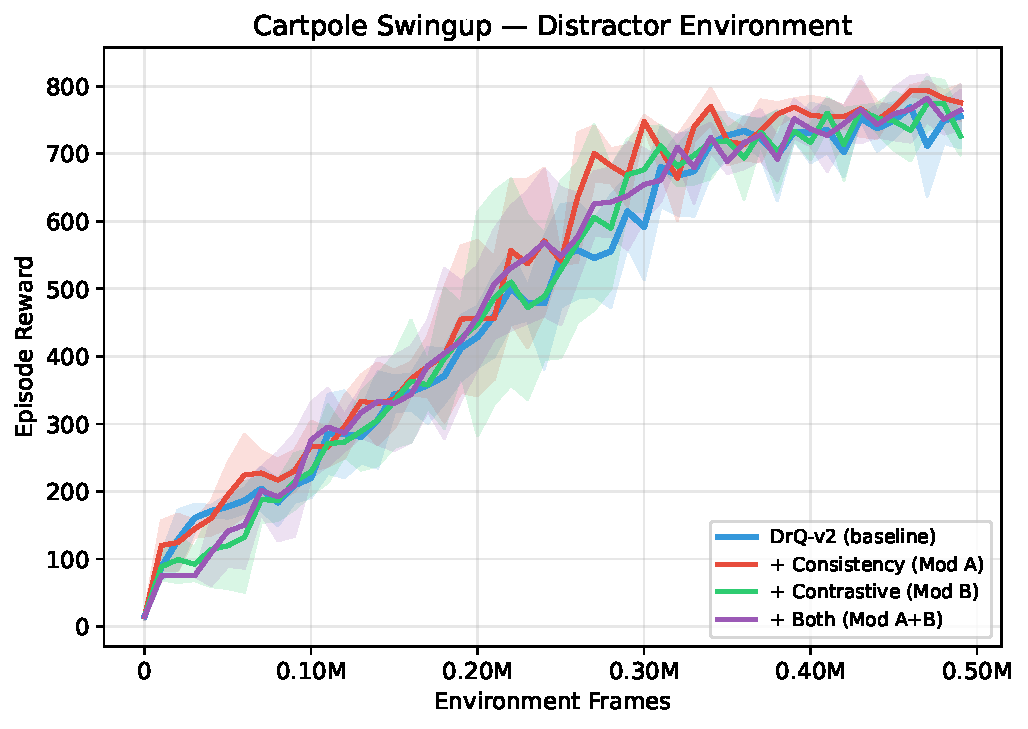
\includegraphics[width=\textwidth]{fig1_distractor_curves.pdf}

\vspace{0.3em}
{\small Distractor setting --- Mod\,A converges\\fastest with tightest confidence bands}
\end{column}
\begin{column}{0.48\textwidth}
\centering
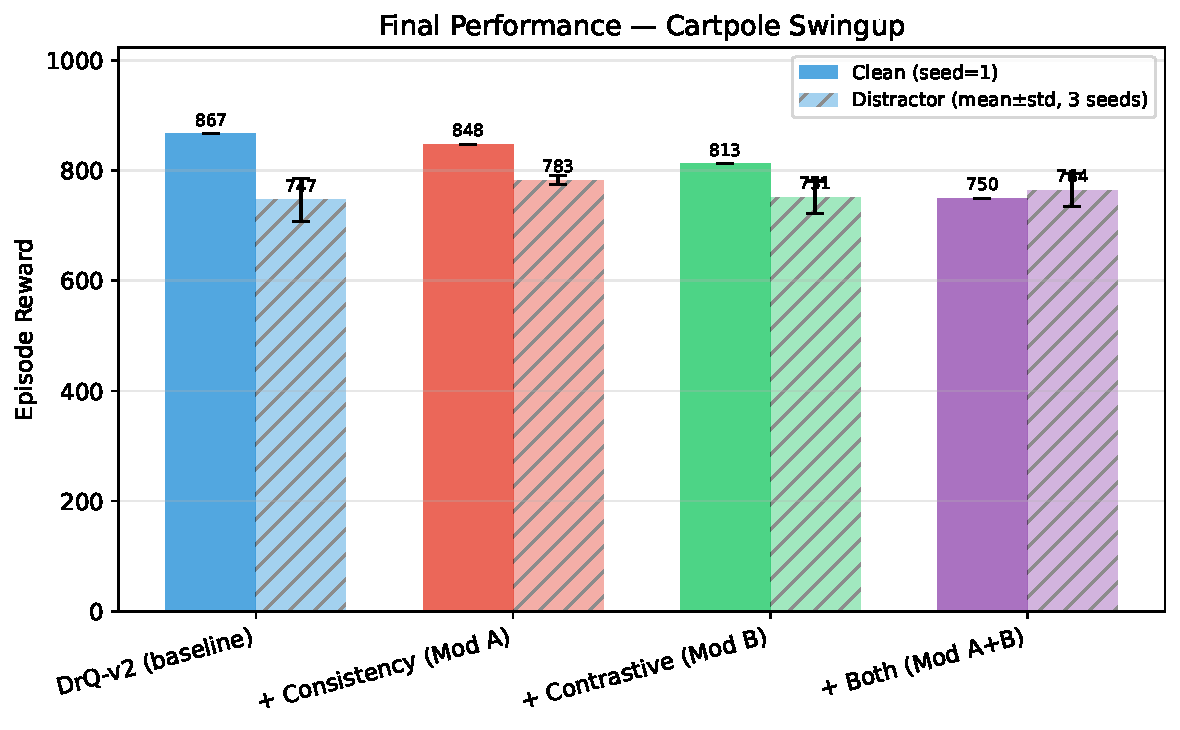
\includegraphics[width=\textwidth]{fig3_final_performance.pdf}

\vspace{0.3em}
{\small Solid = clean, hatched = distractor\\(cartpole: 3-seed mean)}
\end{column}
\end{columns}
\end{frame}

% ==============================================================
\begin{frame}[shrink=5]{Cross-Task Generalization (Seed=1)}
% Speaker: Kean (~50 sec)

\begin{table}
\centering
\renewcommand{\arraystretch}{1.15}
\footnotesize
\begin{tabular}{l cc cc cc}
\toprule
& \multicolumn{2}{c}{\textbf{Cartpole} {\scriptsize(500K)}} & \multicolumn{2}{c}{\textbf{Walker} {\scriptsize(1M)}} & \multicolumn{2}{c}{\textbf{Cheetah} {\scriptsize(1M)}} \\
\cmidrule(lr){2-3} \cmidrule(lr){4-5} \cmidrule(lr){6-7}
\textbf{Method} & Clean & Dist. & Clean & Dist. & Clean & Dist. \\
\midrule
Baseline & $867$ & $702$ & $958$ & $959$ & $743$ & $\mathbf{596}$ \\
\good{+ Mod\,A} & $848$ & $746$ & $\mathbf{968}$ & $947$ & $657$ & $410$ \\
+ Mod\,B & $853$ & $731$ & $964$ & \bad{27} & $\mathbf{773}$ & $626$ \\
+ Mod\,A+B & $750$ & $\mathbf{770}$ & $907$ & $951$ & $705$ & $618$ \\
\bottomrule
\end{tabular}
\end{table}

\vspace{0.2em}
\small
\begin{itemize}\setlength{\itemsep}{1pt}
    \item \good{Mod\,A}: best walker distractor, but \bad{hurts cheetah} ($409.5$ vs.\ $595.6$)
    \item \bad{Mod\,B}: walker distractor collapse ($26.6$), best clean cheetah ($773.2$)
    \item \highlight{No single auxiliary loss dominates all tasks}
\end{itemize}
\end{frame}

% ==============================================================
\begin{frame}{$\alpha$ Sensitivity Ablation (Cartpole)}
% Speaker: Kean (~40 sec)

\begin{columns}[T]
\begin{column}{0.48\textwidth}
\centering
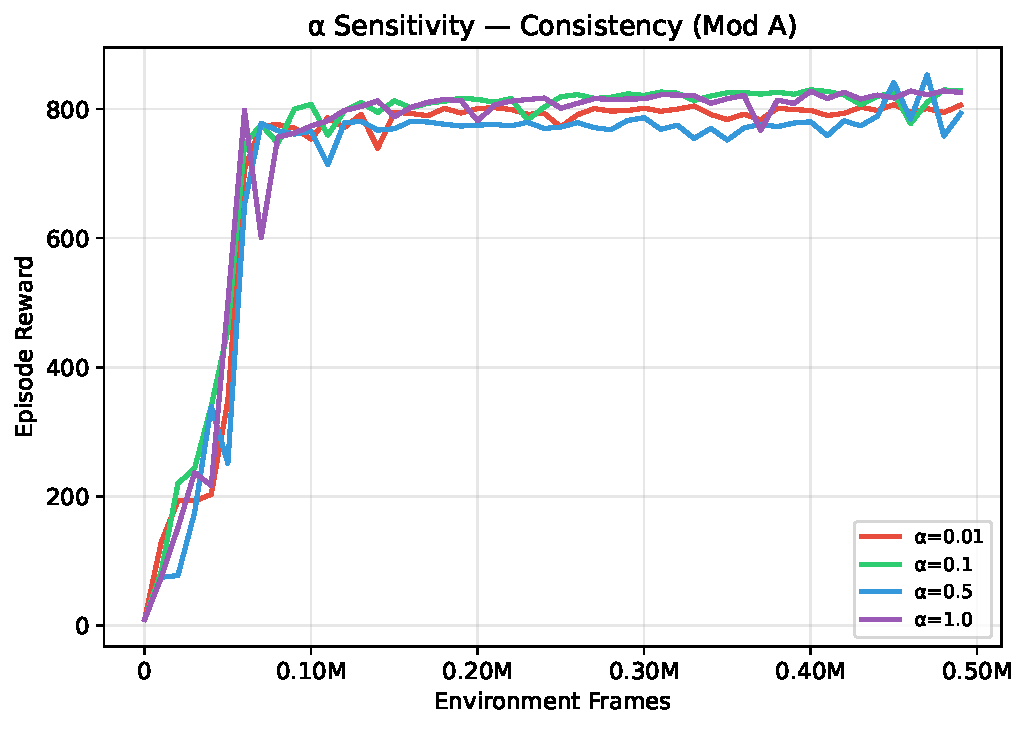
\includegraphics[width=0.92\textwidth]{fig5_alpha_modA.pdf}

\vspace{0.2em}
{\small \good{Mod\,A}: Robust --- all $\alpha \in [0.01, 1.0]$\\converge to $\sim$800--830}
\end{column}
\begin{column}{0.48\textwidth}
\centering
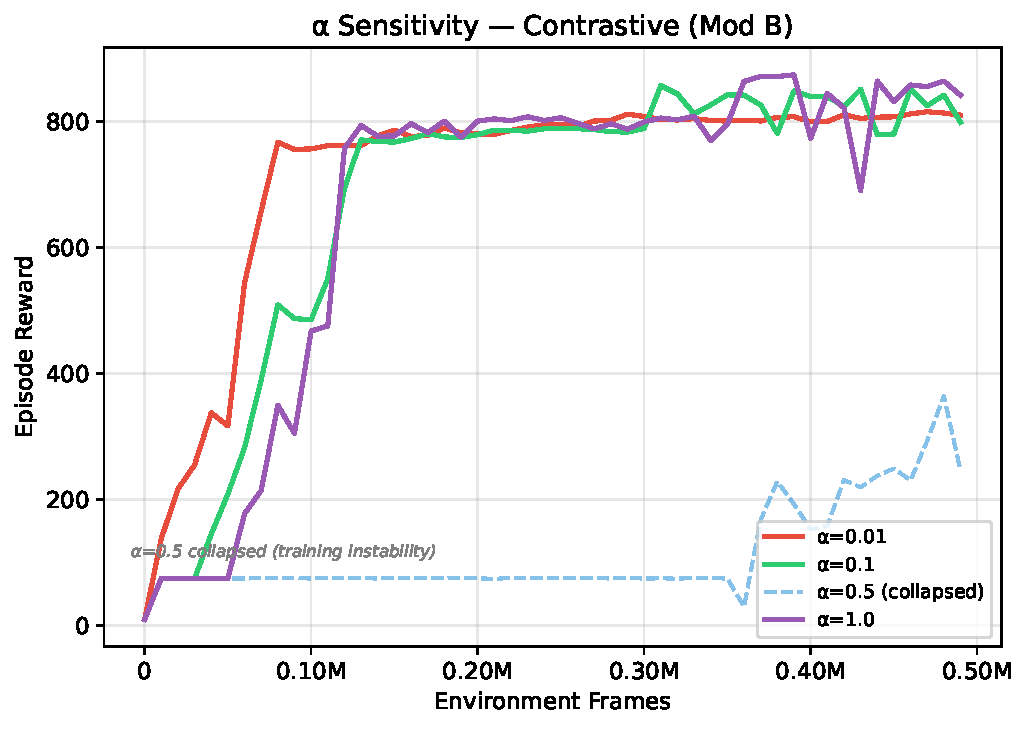
\includegraphics[width=0.92\textwidth]{fig5_alpha_modB.pdf}

\vspace{0.2em}
{\small \bad{Mod\,B}: Fragile --- $\alpha{=}0.5$ collapses\\to $\sim$277; non-monotonic failure}
\end{column}
\end{columns}
\end{frame}

% ==============================================================
\section{Analysis}

\begin{frame}{Representation Analysis: Rank \& Invariance}
% Speaker: Kean (~30 sec)

\begin{columns}[c]
\begin{column}{0.48\textwidth}
\centering
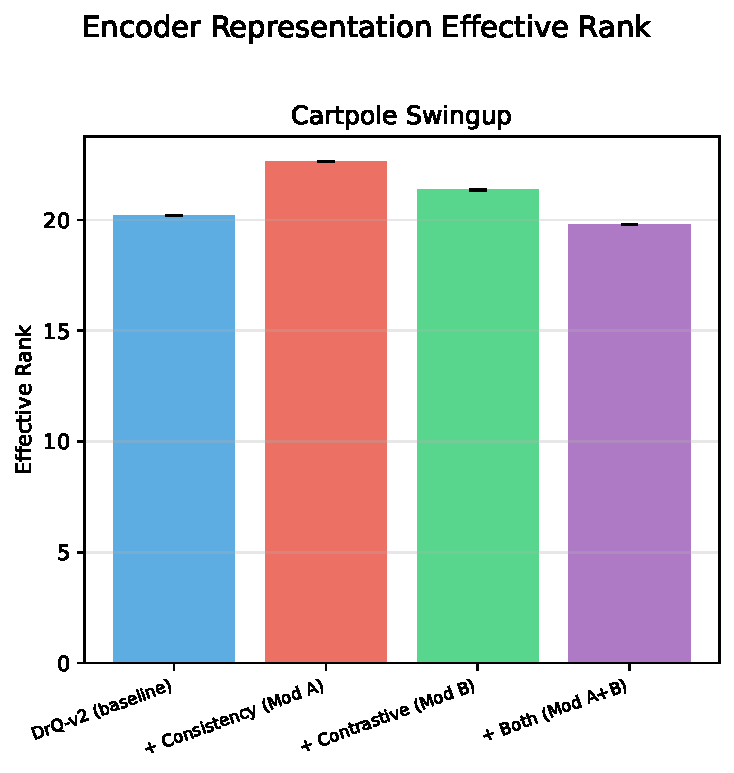
\includegraphics[width=0.65\textwidth]{effective_rank.pdf}

\vspace{0.2em}
{\small\highlight{Effective Rank} (SVD entropy)}\\[0.1em]
{\footnotesize A: \good{22.5} $>$ B: 21.2 $>$ Base: 20.2 $>$ A+B: 19.8}
\end{column}
\begin{column}{0.48\textwidth}
\centering
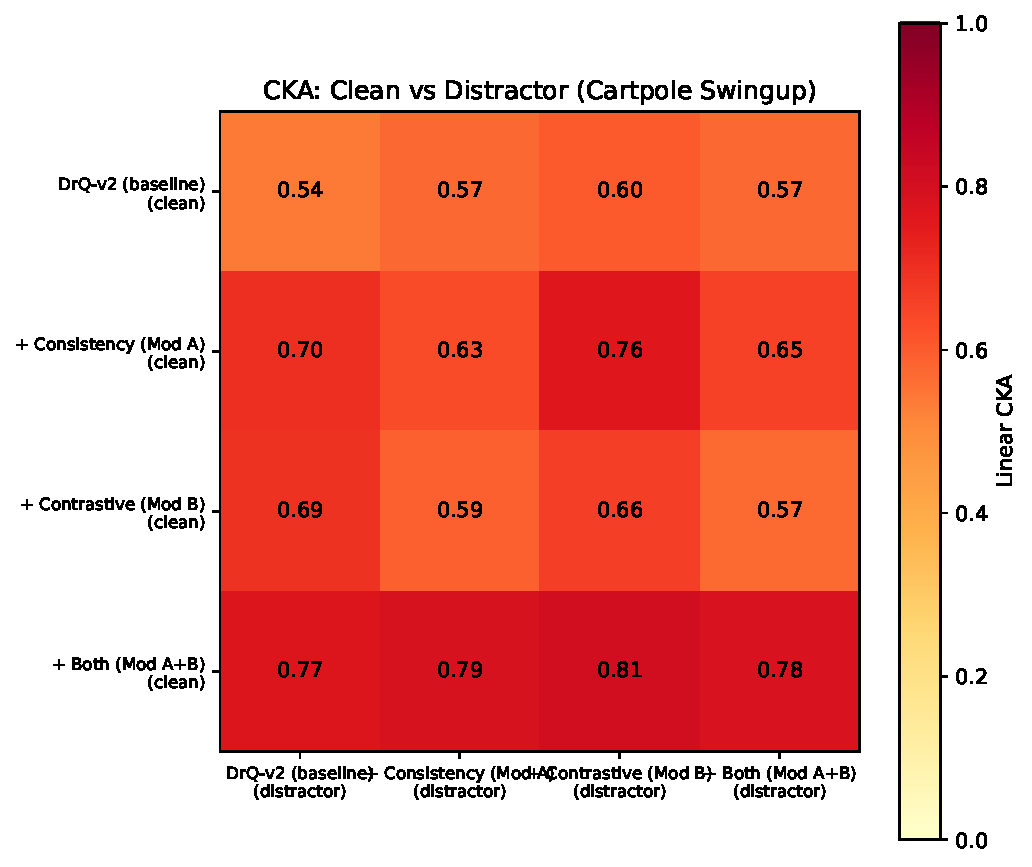
\includegraphics[width=0.65\textwidth]{cka_cartpole_swingup.pdf}

\vspace{0.2em}
{\small\highlight{CKA} (clean--distractor similarity)}\\[0.1em]
{\footnotesize A+B: \good{0.78} $>$ B: 0.66 $>$ A: 0.63 $>$ Base: 0.54}
\end{column}
\end{columns}

\vspace{0.3em}
\centering
{\footnotesize Higher rank = more expressive encoder \quad|\quad Higher CKA = encoder ignores distractors}
\end{frame}

% ==============================================================
\begin{frame}{Representation Analysis: Latent Space (t-SNE)}
% Speaker: Kean (~20 sec)

\begin{columns}[c]
\begin{column}{0.48\textwidth}
\centering
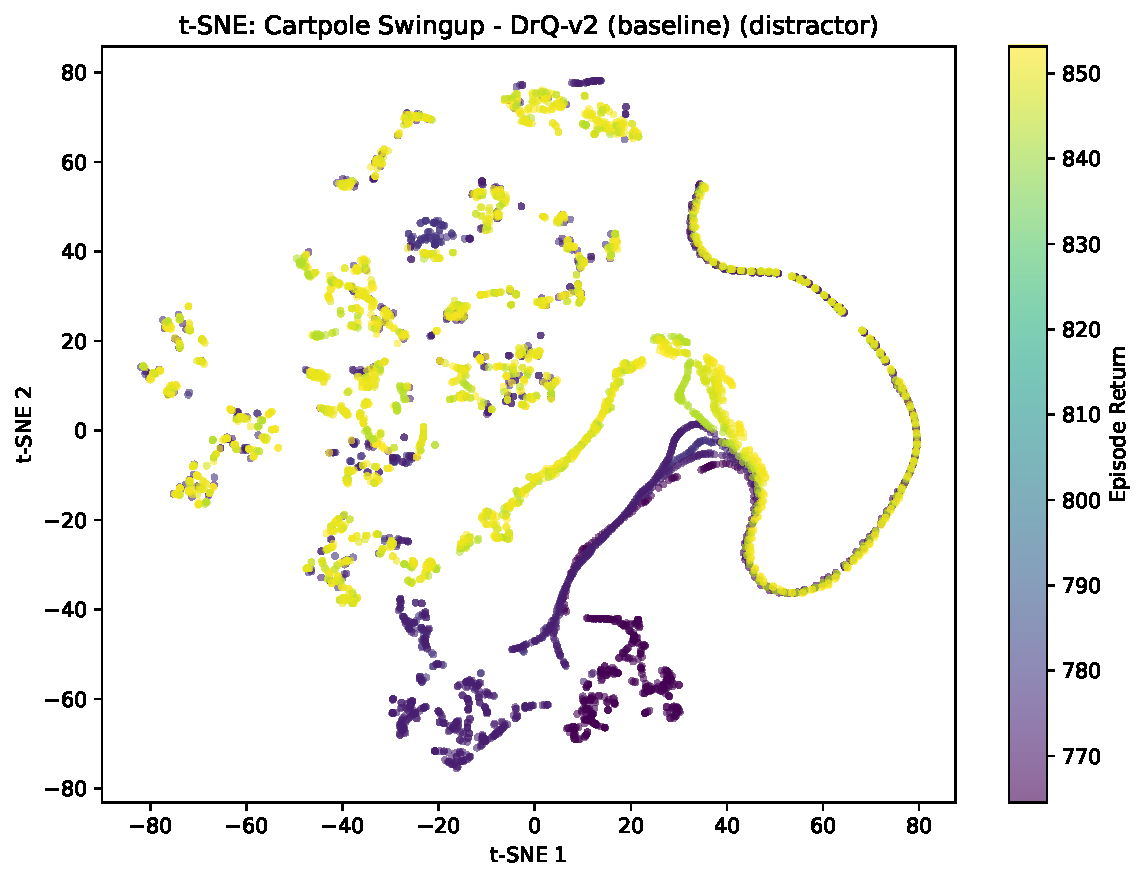
\includegraphics[width=0.65\textwidth]{tsne_cartpole_swingup_baseline_distractor.pdf}

\vspace{0.2em}
{\small\bad{Baseline} (distractor)}\\[0.1em]
{\footnotesize Wide return spread (770--855)}
\end{column}
\begin{column}{0.48\textwidth}
\centering
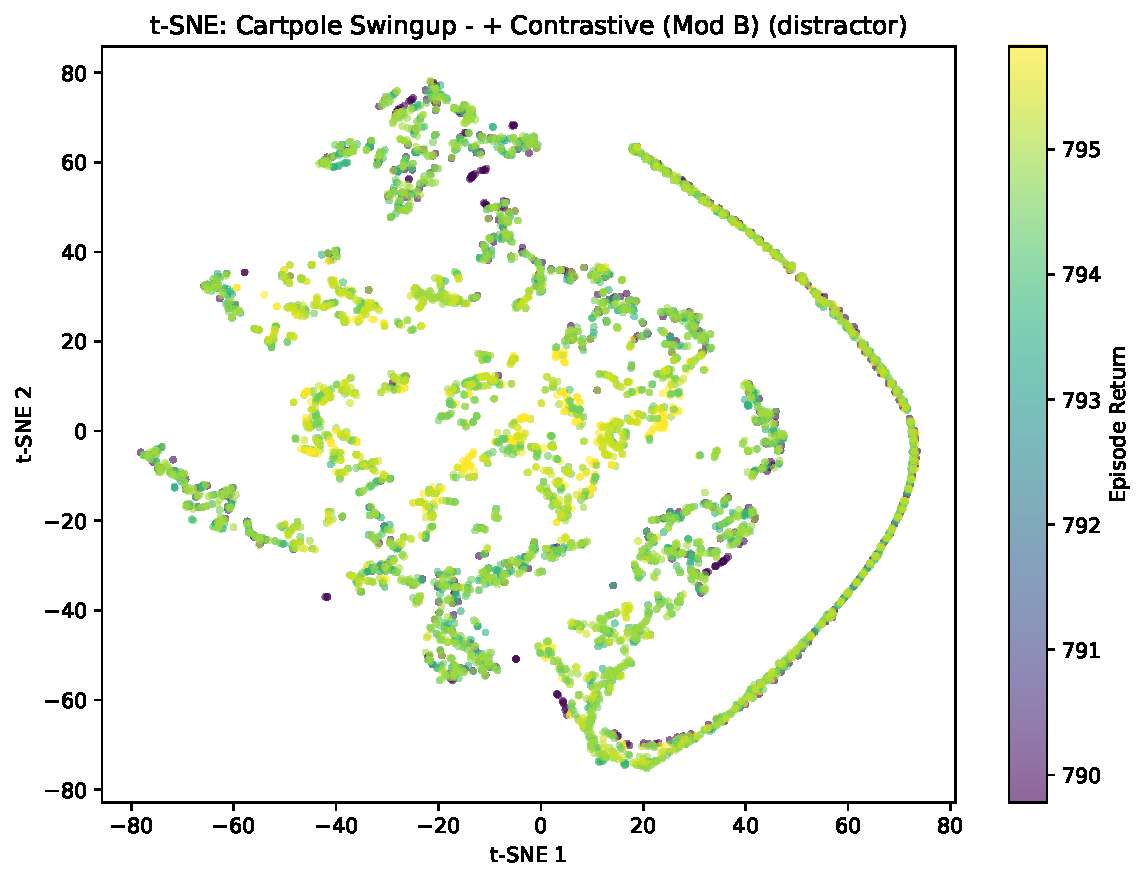
\includegraphics[width=0.65\textwidth]{tsne_cartpole_swingup_modB_distractor.pdf}

\vspace{0.2em}
{\small\good{Mod\,B} (distractor)}\\[0.1em]
{\footnotesize Tight return clustering (790--796)}
\end{column}
\end{columns}

\vspace{0.4em}
\centering
{\small\highlight{Paradox:} Mod\,B produces the best representations, yet is the most unstable method}
\end{frame}

% ==============================================================
\begin{frame}[shrink=5]{Why Mod A Works \& Mod B Fails}
% Speaker: Kean (~45 sec)

\small
\begin{columns}[T]
\begin{column}{0.48\textwidth}
\begin{exampleblock}{\centering Mod\,A --- Recommended}
\begin{itemize}\setlength{\itemsep}{1pt}
    \item \good{Zero overhead}: one MSE term
    \item Highest effective rank ($22.5$)
    \item Robust to $\alpha$: $0.01$--$1.0$
    \item Smallest variance ($\pm 7.8$), $94.4\%$ retention
\end{itemize}
{\footnotesize \textbf{Caveat:} hurts cheetah ($409.5$ vs.\ $595.6$)}
\end{exampleblock}
\end{column}
\begin{column}{0.48\textwidth}
\begin{alertblock}{\centering Mod\,B --- Unstable}
\textbf{Circular dependency:}\\
good pairs $\to$ good Q $\to$ good encoder $\to$ pairs

\vspace{0.1em}
\textbf{Failures:} 1/3 seeds collapsed; $\alpha{=}0.5$ fails; walker: \bad{26.6}
\end{alertblock}
\end{column}
\end{columns}

\vspace{0.2em}
\centering\small
\highlight{Paradox:} A+B has highest CKA (0.78) but \emph{not} highest reward \;$\Rightarrow$\; \textbf{invariance $\neq$ performance}
\end{frame}

% ==============================================================
\section{Conclusion}

\begin{frame}{Conclusion \& Future Work}
% Speaker: Kean (~40 sec)

\small
\begin{columns}[T]
\begin{column}{0.55\textwidth}
\begin{block}{Key Findings}
\begin{enumerate}\setlength{\itemsep}{2pt}
    \item DrQ-v2 drops $\sim$11\% under video distractors
    \item \good{Mod\,A}: best practical choice --- zero overhead, robust $\alpha$
    \item \bad{Mod\,B}: best representations but unstable
    \item No universal auxiliary loss --- task-dependent
    \item Invariance $\neq$ performance
\end{enumerate}
\end{block}
\end{column}
\begin{column}{0.42\textwidth}
\begin{block}{Future Work}
\begin{itemize}\setlength{\itemsep}{2pt}
    \item Adaptive $\alpha$ via Q-confidence
    \item Warm-start Mod\,B after Q converges
    \item High-dimensional manipulation tasks
    \item Real-world distractors (Kinetics)
\end{itemize}
\end{block}
\end{column}
\end{columns}
\end{frame}

% ==============================================================
{
\setbeamertemplate{footline}{}
\begin{frame}[c]
    \centering
    {\Huge \textcolor{UofTBlue}{Thank you for your attention}}

    \vspace{1.5cm}
    \normalsize
    \begin{tabular}{rl}
    \textbf{Bangcheng Wang} & Motivation, Method, Setup \\
    \textbf{Kean Chen} & Results, Analysis, Conclusion \\
    \end{tabular}

    \vspace{1cm}
    {\small Questions?}
\end{frame}
}

\end{document}
